% small.tex
\documentclass[10pt]{beamer}
\usetheme{amcg}
\beamertemplatenavigationsymbolsempty
\renewcommand{\thefootnote}{}
\providecommand{\e}[1]{\ensuremath{\times 10^{#1}}}
\usepackage{mathptmx}
\usepackage{helvet}
\newcommand\TILDE{\char`\~}
\usepackage{listings}
\usepackage{subfigure}

% items enclosed in square brackets are optional
\title[GFD examples]{Summary of the GFD examples}
\subtitle[]{}
\institute{Department of Earth Science and Engineering, Imperial College London}
\author[Sam Parkinson]{\large{Sam Parkinson}}
\date{}


\begin{document}

%--- the titlepage frame -------------------------%
\begin{frame}
  \titlepage
\end{frame}

%-- Overview slide --- %
\section*{Outline}
\begin{frame}
  \frametitle{Outline}
  \tableofcontents
\end{frame}

%-- Add sections and your outline will be created automatically --%
\subsection{The lock--exchange}

% Frame starts a new slide
\begin{frame}
    \frametitle{The lock--exchange}
\begin{itemize}
\item Fluids of different densities (temperature) separated by a barrier. As the barrier is removed, the denser fluid
  collapses under the lighter.
\item Boussinesq flow, control volume discretisation, mesh adaptivity
\item Run time: 10 min.
\end{itemize}

\begin{figure}
\centering
\includegraphics[width=0.45\textwidth]{./lock_exchange/le_basic_0_T}
\caption{Lock-exchange initial temperature (colour) distribution.}
\end{figure}

\end{frame}
%
\begin{frame}
    \frametitle{The lock--exchange}
\begin{figure}[ht]
  \centering
  % For some reason tex4ht doesn't like these images.
  \subfigure[$t = 0\,$s]{\includegraphics[width=0.45\textwidth]{./lock_exchange/le_basic_0_T}}
  \subfigure[$t = 0\,$s]{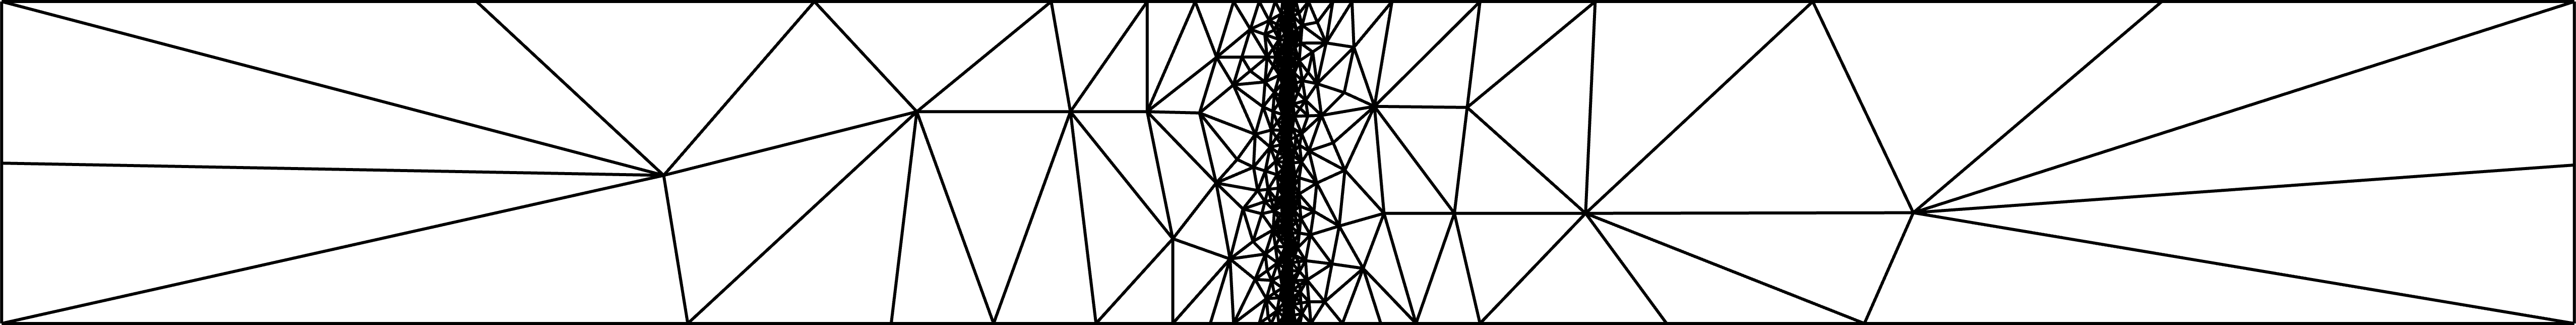
\includegraphics[width=0.45\textwidth]{./lock_exchange/le_basic_0_mesh_nice}} \\
  \subfigure[$t = 12.475\,$s]{\includegraphics[width=0.45\textwidth]{./lock_exchange/le_basic_10_T}}
  \subfigure[$t = 12.475\,$s]{\includegraphics[width=0.45\textwidth]{./lock_exchange/le_basic_10_mesh}} \\
  \subfigure[$t = 37.475\,$s]{\includegraphics[width=0.45\textwidth]{./lock_exchange/le_basic_30_T}}
  \subfigure[$t =
  37.475\,$s]{\includegraphics[width=0.45\textwidth]{./lock_exchange/le_basic_30_mesh}}
  \caption{Lock-exchange temperature distribution (colour) with meshes, over time ($t$).}
\end{figure}
\end{frame}
%
\begin{frame}
    \frametitle{The lock--exchange, diagnostics}
\begin{itemize}
\item Front speed (or Froude number)
\item Mixing given by domain fraction of fluid in specified temperature classes
\end{itemize}

\begin{figure}
\centering
\includegraphics[width=0.5\textwidth]{./lock_exchange/mixing}
\caption{Time evolution of fraction of domain that contains fluid in three temperature classes. Blue: cold, red: warm, green : mixed}
\end{figure}

\end{frame}
%
\begin{frame}
    \frametitle{The lock--exchange, exercises}
\begin{itemize}
\item Increase the simulation time from the default settings (to e.g. 30 secs) and calculate the average Froude number
\item Play with the adaptivity options.
\item Change the diffusivity and viscosity values.
\item Run with a fixed mesh (this will require making a new input mesh)
\item Try adding some detectors to visualise the particle trajectories.
\end{itemize}

\end{frame}

%-- Add sections and your outline will be created automatically --%
\section{Tsunami}

% Frame starts a new slide
\begin{frame}
    \frametitle{Hokkaido-Nansei-Oki tsunami}
\begin{minipage}[]{0.5\linewidth} 
\begin{itemize}
\item Okushiri island, Japan, 1993. 
\item Runup height of up to 30m.
\item Simulation based on a 1:400 laboratory setup.
\item Uses the free-surface and wetting and drying functionality of Fluidity.
\end{itemize}
\end{minipage}
\hspace{0.5cm}
\begin{minipage}[]{0.4\linewidth} 
\begin{figure}
\begin{center}
\includegraphics[width=\textwidth]{hokkaido-nansei-oki_tsunami/MonaiValleyDomainWithInputWave2_png.pdf}
\end{center}
\caption{The domain and the three gauge stations.}\label{fig:monai_inputwave}
\end{figure}
\end{minipage}
\end{frame}

\begin{frame}
    \frametitle{Hokkaido-Nansei-Oki tsunami}
\begin{figure}
\begin{center}
\includegraphics[width=0.7\textwidth]{hokkaido-nansei-oki_tsunami/MonaiValley_C_p1p1_nu0_01_kmkstab_drag0_002_butcircularoundisland0_2-crop-crop_final2.pdf}
\caption{The numerical and experimental results at the three gauge stations.}\label{fig:monai_results}
\end{center}
\end{figure}
% end my slide
\end{frame}


\begin{frame}
    \frametitle{Hokkaido-Nansei-Oki tsunami - Exercises}
  \begin{itemize}
    \item Add more detectors.\newline
    \item Check how increasing the wetting and drying threshold parameter affects the results.\newline
    \item Try changing the viscosity value (How does it affect the inundation of the tsunami event?).
  \end{itemize}
% end my slide
\end{frame}



%-- Add sections and your outline will be created automatically --%
\subsection{Rotating periodic channel}

% Frame starts a new slide
\begin{frame}
    \frametitle{Rotating periodic channel}
\begin{itemize}
\item Unit square domain, periodic in zonal direction and zero-slip at North and South boundaries.  Coriolis forcing.
\item The flow is driven by a velocity source term:
\begin{equation*}
  \vec{F}=
  \begin{bmatrix}
    y^3 \\
    0
  \end{bmatrix}
\end{equation*}
\item Provides a convergence test for the $P_{1DG}P_2$ element pair.
\item A good example of using python state for online diagnostics and analysis, and also using python for setting initial conditions.
\item Run time: 10 min. 
\end{itemize}
\end{frame}
%
\begin{frame}
    \frametitle{Rotating periodic channel}
\begin{figure}
\includegraphics[width=0.6\textwidth]{./rotating_channel/analytic_solution}
\caption{Velocity forcing term and analytic solutions for velocity and pressure for the rotating periodic channel test case. Note that each of these quantities is constant in the x direction.}
\end{figure}
\end{frame}
%
\begin{frame}
    \frametitle{Rotating periodic channel}
\begin{figure}
\includegraphics[width=0.6\textwidth]{./rotating_channel/convergence}
\caption{Error in the pressure and velocity solutions for the rotating channel as a function of resolution.}
\end{figure}
\end{frame}
%
\begin{frame}
    \frametitle{Rotating periodic channel, exercises}
\begin{itemize}
\item Understand the use of analytic forcing functions in Fluidity using Python.
\item For the Continuous Galerkin example, see what the effect is of removing the SUPG stabilisation
\item Change the resolution of the adapted meshes
\item Change the spatial and temporal discretisations to get a less diffusive advection scheme
\end{itemize}
\end{frame}


%-- Add sections and your outline will be created automatically --%
\section{Restratification following open ocean deep convection}

% Frame starts a new slide
\begin{frame}
    \frametitle{Restratification following open ocean deep convection}
\begin{itemize}
\item Idealised model of the restratification phase of OODC using $P_1DGP_2$ using an extruded mesh.
\end{itemize}
\begin{figure}
\includegraphics[width=0.5\textwidth]{./restratification_after_oodc/rousset-init.png}
\caption{A vertical slice throughout the domain showing the initial temperature stratification. The domain is a cylinder of radius $250 \,$km and height $1\,$km.}
\end{figure}
\end{frame}
%
\begin{frame}
    \frametitle{Restratification following open ocean deep convection}
\begin{figure}
\centering
\subfigure [0 days]{\includegraphics[width=0.175\textwidth]{./restratification_after_oodc/rousset-res5000-depth-40m0001.png}}
\subfigure [10 days]{\includegraphics[width=0.175\textwidth]{./restratification_after_oodc/rousset-res5000-depth-40m0003.png}}
\subfigure [20 days]{\includegraphics[width=0.175\textwidth]{./restratification_after_oodc/rousset-res5000-depth-40m0005.png}}
\subfigure [30 days]{\includegraphics[width=0.175\textwidth]{./restratification_after_oodc/rousset-res5000-depth-40m0007.png}}
\subfigure [40 days]{\includegraphics[width=0.175\textwidth]{./restratification_after_oodc/rousset-res5000-depth-40m0009.png}}
\caption{The temperature cross section at a depth of $40\,$m.}
\end{figure}
\end{frame}
%
\begin{frame}
    \frametitle{Restratification following open ocean deep convection, exercises}
\begin{itemize}
\item Work out the kinetic and potential energies using the vtus or stat file.
\item Try running with different resolutions and look at the effect on the eddies.
\end{itemize}
\end{frame}


%-- Add sections and your outline will be created automatically --%
\section{Tides in the Mediterranean Sea}

% Frame starts a new slide
\begin{frame}
    \frametitle{Tides in the Mediterranean Sea}
\begin{itemize}
\item Tidal modelling is a widely used method for validating free surface implementations.
\item Tides introduced by an astronomical body forcing, and a
\item Co--oscillating boundary tide forcing.
\item This example considers the four main tidal constituents: \mbox{$M_2, \, S_2, \, K_1 \,\, {\rm and} \,\, O_1$}.
\end{itemize}
\end{frame}
%
\begin{frame}
    \frametitle{Tides in the Mediterranean Sea}
\begin{figure}
\centering
\includegraphics[width=0.9\textwidth, clip = True, trim = 5mm 180mm 0mm 0mm]{./tides_in_the_Mediterranean_Sea/amp.png}
\caption{The $M_2$ tidal harmonic amplitude from (left) Fluidity--ICOM and (right) a high resolution tidal model${}^\dagger$.}
\end{figure}
\footnote{${}^\dagger$ M.~N.~Tsimplis {\it et al.} (1995), J. Geophys. Res. 100 (C8).}
\end{frame}
%

\begin{frame}
    \frametitle{Tides in the Mediterranean Sea}
The amplitude of each of the todal components is considered, and a RMS error of the difference of these to observed tide guage data is calculated.  The locations of these tide guages is shown below.
\begin{figure}
\centering
\includegraphics[width=0.6\textwidth]{./tides_in_the_Mediterranean_Sea/gauges.png}
\caption{Locations of 62 tide gauges in the Mediterranean Sea used to calculate the root mean square error.}
\end{figure}
\end{frame}


\begin{frame}
    \frametitle{Tides in the Mediterranean Sea - exercises}
\centering
\begin{itemize}
\item Consider the forcing tidal components contained in the netCDF file 'med.nc' (e.g. using ncview).
\item Examine the mesh features (e.g. open the '.msh' file in Gmsh).
\item Look at how to apply the forcing of different tidal components in the simulation.
\item Limit the error calculation by region, are the errors greater in some parts of the Mediterranean?
\end{itemize}
\end{frame}

%-- Add sections and your outline will be created automatically --%
\section{Stokes square convection}

% Frame starts a new slide
\begin{frame}
    \frametitle{Stokes square convection}
\begin{itemize}
\item A steady–state isoviscous convection at a Rayleigh number (Ra) of $10^5$ , in a
  two dimensional square domain of unit dimensions 
\item comparison of numerical results against a well established two dimensional cartesian geometry
  benchmark result for Stokes flow
\end{itemize}
\end{frame}

\begin{frame}
    \frametitle{Stokes square convection}
\begin{figure}
  \includegraphics[width=0.5\textwidth]{./stokes_square_convection/Temperature_planform.png}
  \caption{Steady–state temperature field from an isoviscous Stokes simulation at $Ra = 1 \times
    10^5$, on a uniform structured mesh of 48 × 48 elements. Contours are spaced at intervals of
    0.1.}
\end{figure}
\end{frame}
%
\begin{frame}
    \frametitle{Stokes square convection}
\begin{figure}
\centering
\includegraphics[width=0.5\textwidth]{./stokes_square_convection/Nu_1e5.png}
\includegraphics[width=0.5\textwidth]{./stokes_square_convection/RMS_1e5.png}
\caption{Results from 2-D, isoviscous Stokes square convection benchmark cases: (a) Nusselt number
  vs. number of triangle vertices, at $Ra = 1 \times 10^5$, (b) RMS velocity vs. number of triangle
  vertices, at $Ra = 1 \times 10^5$ . Benchmark values are denoted by horizontal dashed lines. Note that the
  highest resolution case is not included in the example.}
\end{figure}
\end{frame}
%
\begin{frame}
    \frametitle{Stokes square convection, exercises}
\begin{itemize}
\item Verify that results do indeed converge towards the benchmark values at higher resolution.
\item Alter the initial condition for temperature to verify that, excluding the location of upwelling
flow at $x = 0$ or $x = 1$, results are insensitive to this initial condition.
\item Change the Rayleigh number to $Ra = 1 \times 10^4$
\end{itemize}
\end{frame}



%-- Data directory slide --- %
\section*{Data}
\begin{frame}
  \frametitle{Data}
  \begin{center}
  The examples have been run in advance \\ and the output can be found in \\ /scratch/release-examples
  \end{center}
\end{frame}

\end{document}




